In Abbildung \ref{fig:bild} ist ein typisches Signalbild dargestellt.
Auf der X-Achse ist das Magnetfeld aufgetragen, auf der Y-Achse die Transparenz des Rb-Dampfes.
Das Minimum auf der linken Seite entsteht dadurch, dass dort kein Magnetfeld anliegt und es so auch zu keiner Zeemanaufspaltung kommen kann.
Die beiden Resonanzstellen enstehen durch die gegebenen Isotope $R^{87}$ und $R^{85}$.
Im Folgenden wird die Zuordnung der Isotope zu den Minima vorgenommen.
Bis zu dem Zeitpunkt werden die Minnima mit 1 und 2 (von Links nach Rechts) bezeichnet.
\begin{figure}[h!]
  \centering
  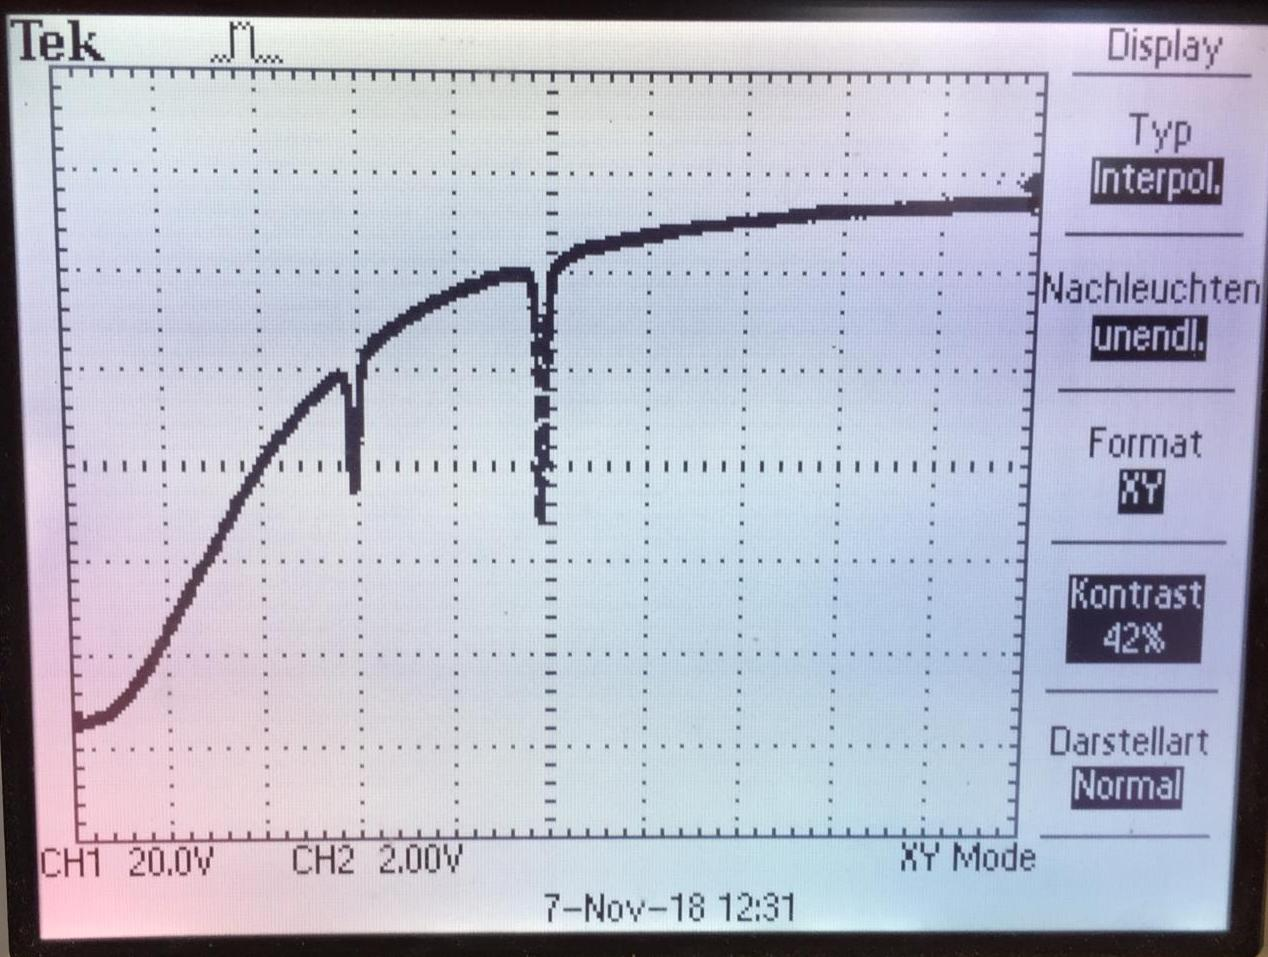
\includegraphics[width=0.8\textwidth]{bild.jpeg}
  \caption{Das für die Resonanzstelle benötigte Magnetfeld aufgetragen auf die Frequenz}
  \label{fig:bild}
\end{figure}
Anhand der Abbildung \ref{fig:bild} kann eine Abschätzung des prozentualen Verhältnisses der beiden Isotope getroffen werden.
Dabei gilt:
\begin{align*}
  N_1+N_2 = 1
\end{align*}
$N$ beschreibt dabei den prozentualen Anteil des Iostopes an der Gesamtanzahl.
Durch Ausmessen der Minima ergibt sich ein Verhältniss $R$ für $\frac{N_1}{N_2}$ von:
\begin{align*}
  R=\SI{0.48}{}
\end{align*}
Die Anteile $N$ lassen sich bestimmen zu:
\begin{align*}
  N_1&=\frac{0,48}{1+0,48}=0,32\\
  N_2&=1-N_1=0,68.
\end{align*}


Um die Resonanzstellen zu erreichen können die Potentiometer für die Horizontale Spule und für die Sweep-Spule variiert werden.
Die zur jeweiligen Resonanzstelle gehörigen Potentiometerumdrehungen können wie folgt in eine Stromstärke $I$ umgerechnet werden.
\begin{align*}
  \text{Sweep-Spule}&&&\text{Horizontale Spule}\\
  \SI{1}{Umdrehung} &= \SI{0,1}{A}&&\SI{1}{Umdrehung} = \SI{0,3}{A}
\end{align*}
Aus den resultierenden Stromstärken kann das B-Feld berrechnet werden.
\begin{align*}
  B=\mu_0\frac{8}{\sqrt{125}}\frac{N\cdot I}{R}
\end{align*}
Die Windungszahl $N$ und der Radius $R$ sind dabei spulenspezifische Größen.
\begin{align*}
  &\text{Sweep-Spule}&&\text{Horizontale Spule}\\
  &N=11&&N=154\\
  &R=\SI{0.1639}{m}&&R=\SI{0.1579}{m}\\
\end{align*}
Die $B$-Felder von der Sweep-Spule $B_S$ und der Horizontalspule $B_H$ für eine Resonanzstelle müssen anschließend addiert werden um das gesamte Magnetfeld $B_{\text{ges}}$ zu erhalten.
Die errechnete Werte für Stromstärke $I$ und $B$-Feld sind zusammen mit den dazugehörigen Frequenzen in der Tabelle \ref{tab:Tab1} aufgeführt.
\begin{table}
  \centering
  \caption{In Abhängigkeit der eingestellten Frequenz aufgenommene Stromstärken durch die beiden Horizontalspulen. Aufgenommen wurden die Stromstärke an den Resonanzstellen für die beiden Isotope (1) und (2), mit dem gegebenen Maßen der Spulen wurde das horizontale Gesamtfeld aus den Stromstärken bestimmt.}
  \label{tab.Tab1}
    \begin{tabular}{c c c c c c c}
      \toprule
      Frequenz  & Stromstärke & Stromstärke & B-Feld 1 & Stromstärke & Stromstärke &  B-Feld 2\\
        & Horizontalspule & Sweep-Spule & & Horizontalspule & Sweep-Spule&\\
      kHz & A& A& $\mu$T & A& A& $\mu$T\\
      \midrule
      \midrule
      100     & 0,000  &  0,501 &  30,234  &  0,000 &  0,621 &  37,476 \\
      200     & 0,024  &  0,432 &  47,117  &  0,024 &  0,677 &  61,902 \\
      300     & 0,045  &  0,451 &  66,680  &  0,045 &  0,833 &  89,733 \\
      400     & 0,060  &  0,400 &  76,757  &  0,060 &  0,880 & 105,724 \\
      500     & 0,081  &  0,324 &  90,587  &  0,081 &  0,907 & 125,769 \\
      600     & 0,093  &  0,390 & 105,093  &  0,111 &  0,824 & 147,069 \\
      700     & 0,111  &  0,342 & 117,982  &  0,138 &  0,769 & 167,429 \\
      800     & 0,114  &  0,549 & 133,105  &  0,180 &  0,510 & 188,631 \\
      900     & 0,138  &  0,440 & 147,574  &  0,204 &  0,544 & 211,730 \\
      1000    & 0,144  &  0,617 & 163,518  &  0,234 &  0,503 & 235,565 \\
      \bottomrule
    \end{tabular}
\end{table}

In der Graphik \ref{fig:Bf} sind die Werte graphisch dagestellt.
\begin{figure}[h!]
  \centering
  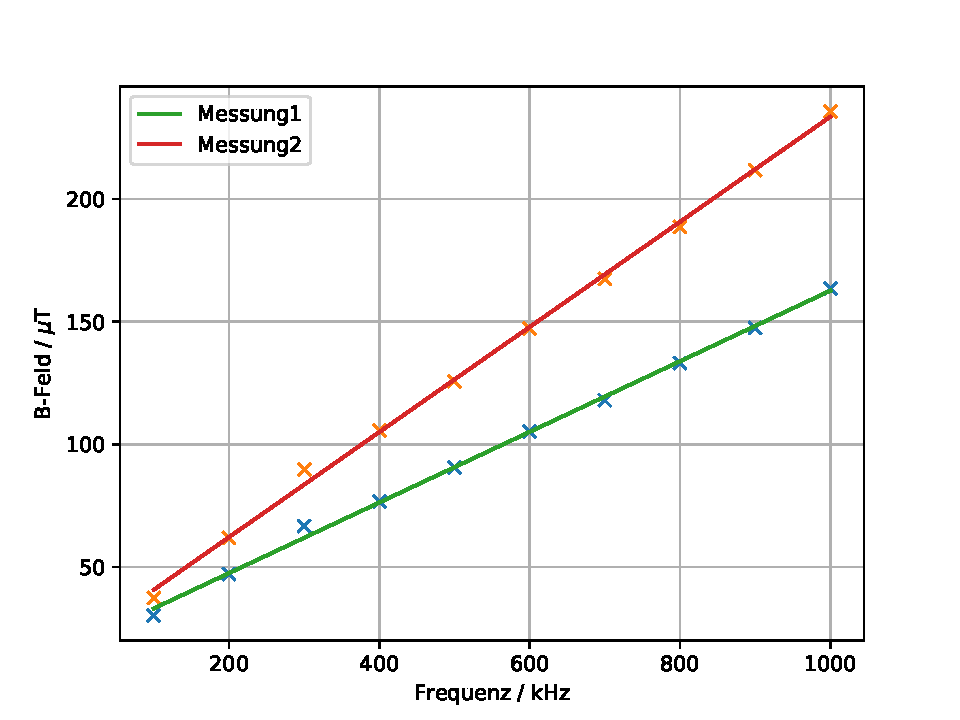
\includegraphics[width=\textwidth]{B-Feld.pdf}
  \caption{Das für die Resonanzstelle benötigte Magnetfeld aufgetragen auf die Frequenz}
  \label{fig:Bf}
\end{figure}
Es wird eine Ausgleichsrechnung der Form:
\begin{align*}
  B(f)=a_if+b_i
\end{align*}
durchgeführt.
Es ergeben sich folgende Fit-Parameter:
\begin{align*}
  a_1&=\SI{1.438\pm 0.023e-10}{\frac{T}{Hz}}\\
  b_1&=\SI{1.876\pm 0.144e-5}{T}
\end{align*}
\begin{align*}
  a_2&=\SI{2.141\pm0.031e-10}{\frac{T}{Hz}}\\
  b_2&=\SI{1.935\pm0.190e-5}{T}
\end{align*}
\FloatBarrier
Mit der Steigung $a$ kann der Landesche $g_F$-Faktor mit der Gleichung $\ref{eqn:landef}$wie folgt bestimmt werden.
\begin{align*}
  g_F = \frac{h}{\mu_0\cdot a_i}
\end{align*}
Somit ergeben sich die Landeschen Faktoren zu:
\begin{align*}
  g_{F1} = 0,497\pm0,008\\
  g_{F2} = 0,334\pm0,004.
\end{align*}

Nun soll der Kernspinn bestimmt werden.

Die den für den Versuch wichtigen Quantenzahlen lauten:
\begin{equation}
	S = \frac{1}{2},\quad L = 0,\quad J = \frac{1}{2},\quad F = I + J.
\end{equation}
wobei $F$ den höchst mögliche Wert besitzt da nur für das Niveau mit dem höchst möglichen $m_F$
kein Übergang mit $\Delta m_{f}$ mehr möglich ist. Eingesetzt in die Gleichung:
\begin{align}
	g_F\approx g_J\frac{F\cdot(F+1)+J\cdot(J+1)-I(I+1)}{2F\cdot(F+1)}
	\label{eq:lande_faktor_gf}
\end{align}
ergibt sich die Formel für den Kernspin:
\begin{align*}
  I = \frac{1}{2}\left(\frac{g_J}{g_F}-1\right).
\end{align*}

Das benötigte $g_J$ kann mit Hilfe von $\ref{eqn:landej}$ besimmt werden.
Dabei ist $g_s$ gegeben als
\begin{align*}
  g_s = 2,0023
\end{align*}

Es lässt sich die Relation aufstellen:
\begin{align*}
  g_J=g_s.
\end{align*}

Der Kernspin kann jetzt bestimmt werden.
\begin{align*}
  I_1=1,5153\pm0,03\\
  I_2=2,4999\pm0,04
\end{align*}
Durch einen Vergleich mit Literaturwerten \cite{Spin} kann der Kernspinn den Rubidium-Isotopen zugeordnet werden.
Es gilt:
\begin{align*}
  I_{Rb^{85}}=\frac{5}{2}\\
  I_{Rb^{87}}=\frac{3}{2}
\end{align*}
Es wird deutlich, dass
\begin{align*}
  I_1=I_{Rb^{87}}\\
  I_2=I_{Rb^{85}}
\end{align*}
gilt.\\

Mit Hilfe der Formel \ref{eqn:quadzeeman} kann der lineare und der quadratische Zeeman-Effekt bestimmt werden.
In der Tabelle \ref{tab.QZ} sind die Werte für den lineare und den quadratische Zeeman-Effekt abgebildet.
Es wird deutlich, dass der qudratische Zeeman-Effekt im verglich zum linearen vernachlässigbar klein ist.
\FloatBarrier

\begin{table}
  \centering
  \caption{Der Quadratische Zeemaneffekt zu den beiden Isotopen}
  \label{tab.QZ}
    \begin{tabular}{c c c}
      \toprule
        & Linearer Zeeman    &Quadratischer Zeeman\\
        %& \si{J} & \si{J} \\
      \midrule
      \midrule
      $U_{85}$ & $\SI{5.05e-28}{J}$ & $-6,35\cdot 10^{-31}\si{J}$\\
      $U_{87}$ & $\SI{1.09e-27}{J}$ & $-7,86\cdot 10^{-31}\si{J}$\\
      \bottomrule
    \end{tabular}
\end{table}


%Die errechneten Weren sind in der Tabelle \ref{tab.QZ} für die beiden Isotope aufgefürt.
%\begin{table}
  \centering
  \caption{Der Quadratische Zeemaneffekt zu den beiden Isotopen}
  \label{tab.QZ}
    \begin{tabular}{c c c c c}
      \toprule
      Frequenz  &  B-Feld 1 & Quad. Zeeman  & B-Feld 2  &Quad. Zeeman\\
      kHz & $\mu$T & 1$\cdot10^{-20}$ & $\mu$T  & 1$\cdot10^{-20}$ \\
      \midrule
      \midrule
      100     &   30,234 &  -1,271\pm0,021   &  37,476  &   -1,998\pm0,029     \\
      200     &   47,117 &  -3,099\pm0,050   &  61,902  &   -5,464\pm0,078     \\
      300     &   66,680 &  -6,219\pm0,100   &  89,733  &  -11,491\pm0,164     \\
      400     &   76,757 &  -8,246\pm0,133   & 105,724  &  -15,957\pm0,228     \\
      500     &   90,587 & -11,493\pm0,185   & 125,769  &  -22,587\pm0,323     \\
      600     &  105,093 & -15,477\pm0,250   & 147,069  &  -30,891\pm0,442     \\
      700     &  117,982 & -19,512\pm0,315   & 167,429  &  -40,041\pm0,573     \\
      800     &  133,105 & -24,843\pm0,401   & 188,631  &  -50,829\pm0,727     \\
      900     &  147,574 & -30,545\pm0,493   & 211,730  &  -64,047\pm0,916     \\
      1000    &  163,518 & -37,510\pm0,605   & 235,565  &  -79,284\pm0,113     \\
      \bottomrule
    \end{tabular}
\end{table}

